% Options for packages loaded elsewhere
\PassOptionsToPackage{unicode}{hyperref}
\PassOptionsToPackage{hyphens}{url}
\PassOptionsToPackage{dvipsnames,svgnames,x11names}{xcolor}
%
\documentclass[
  letterpaper,
  DIV=11,
  numbers=noendperiod]{scrartcl}

\usepackage{amsmath,amssymb}
\usepackage{iftex}
\ifPDFTeX
  \usepackage[T1]{fontenc}
  \usepackage[utf8]{inputenc}
  \usepackage{textcomp} % provide euro and other symbols
\else % if luatex or xetex
  \usepackage{unicode-math}
  \defaultfontfeatures{Scale=MatchLowercase}
  \defaultfontfeatures[\rmfamily]{Ligatures=TeX,Scale=1}
\fi
\usepackage{lmodern}
\ifPDFTeX\else  
    % xetex/luatex font selection
\fi
% Use upquote if available, for straight quotes in verbatim environments
\IfFileExists{upquote.sty}{\usepackage{upquote}}{}
\IfFileExists{microtype.sty}{% use microtype if available
  \usepackage[]{microtype}
  \UseMicrotypeSet[protrusion]{basicmath} % disable protrusion for tt fonts
}{}
\makeatletter
\@ifundefined{KOMAClassName}{% if non-KOMA class
  \IfFileExists{parskip.sty}{%
    \usepackage{parskip}
  }{% else
    \setlength{\parindent}{0pt}
    \setlength{\parskip}{6pt plus 2pt minus 1pt}}
}{% if KOMA class
  \KOMAoptions{parskip=half}}
\makeatother
\usepackage{xcolor}
\setlength{\emergencystretch}{3em} % prevent overfull lines
\setcounter{secnumdepth}{-\maxdimen} % remove section numbering
% Make \paragraph and \subparagraph free-standing
\makeatletter
\ifx\paragraph\undefined\else
  \let\oldparagraph\paragraph
  \renewcommand{\paragraph}{
    \@ifstar
      \xxxParagraphStar
      \xxxParagraphNoStar
  }
  \newcommand{\xxxParagraphStar}[1]{\oldparagraph*{#1}\mbox{}}
  \newcommand{\xxxParagraphNoStar}[1]{\oldparagraph{#1}\mbox{}}
\fi
\ifx\subparagraph\undefined\else
  \let\oldsubparagraph\subparagraph
  \renewcommand{\subparagraph}{
    \@ifstar
      \xxxSubParagraphStar
      \xxxSubParagraphNoStar
  }
  \newcommand{\xxxSubParagraphStar}[1]{\oldsubparagraph*{#1}\mbox{}}
  \newcommand{\xxxSubParagraphNoStar}[1]{\oldsubparagraph{#1}\mbox{}}
\fi
\makeatother


\providecommand{\tightlist}{%
  \setlength{\itemsep}{0pt}\setlength{\parskip}{0pt}}\usepackage{longtable,booktabs,array}
\usepackage{calc} % for calculating minipage widths
% Correct order of tables after \paragraph or \subparagraph
\usepackage{etoolbox}
\makeatletter
\patchcmd\longtable{\par}{\if@noskipsec\mbox{}\fi\par}{}{}
\makeatother
% Allow footnotes in longtable head/foot
\IfFileExists{footnotehyper.sty}{\usepackage{footnotehyper}}{\usepackage{footnote}}
\makesavenoteenv{longtable}
\usepackage{graphicx}
\makeatletter
\def\maxwidth{\ifdim\Gin@nat@width>\linewidth\linewidth\else\Gin@nat@width\fi}
\def\maxheight{\ifdim\Gin@nat@height>\textheight\textheight\else\Gin@nat@height\fi}
\makeatother
% Scale images if necessary, so that they will not overflow the page
% margins by default, and it is still possible to overwrite the defaults
% using explicit options in \includegraphics[width, height, ...]{}
\setkeys{Gin}{width=\maxwidth,height=\maxheight,keepaspectratio}
% Set default figure placement to htbp
\makeatletter
\def\fps@figure{htbp}
\makeatother
% definitions for citeproc citations
\NewDocumentCommand\citeproctext{}{}
\NewDocumentCommand\citeproc{mm}{%
  \begingroup\def\citeproctext{#2}\cite{#1}\endgroup}
\makeatletter
 % allow citations to break across lines
 \let\@cite@ofmt\@firstofone
 % avoid brackets around text for \cite:
 \def\@biblabel#1{}
 \def\@cite#1#2{{#1\if@tempswa , #2\fi}}
\makeatother
\newlength{\cslhangindent}
\setlength{\cslhangindent}{1.5em}
\newlength{\csllabelwidth}
\setlength{\csllabelwidth}{3em}
\newenvironment{CSLReferences}[2] % #1 hanging-indent, #2 entry-spacing
 {\begin{list}{}{%
  \setlength{\itemindent}{0pt}
  \setlength{\leftmargin}{0pt}
  \setlength{\parsep}{0pt}
  % turn on hanging indent if param 1 is 1
  \ifodd #1
   \setlength{\leftmargin}{\cslhangindent}
   \setlength{\itemindent}{-1\cslhangindent}
  \fi
  % set entry spacing
  \setlength{\itemsep}{#2\baselineskip}}}
 {\end{list}}
\usepackage{calc}
\newcommand{\CSLBlock}[1]{\hfill\break\parbox[t]{\linewidth}{\strut\ignorespaces#1\strut}}
\newcommand{\CSLLeftMargin}[1]{\parbox[t]{\csllabelwidth}{\strut#1\strut}}
\newcommand{\CSLRightInline}[1]{\parbox[t]{\linewidth - \csllabelwidth}{\strut#1\strut}}
\newcommand{\CSLIndent}[1]{\hspace{\cslhangindent}#1}

\KOMAoption{captions}{tableheading}
\makeatletter
\@ifpackageloaded{caption}{}{\usepackage{caption}}
\AtBeginDocument{%
\ifdefined\contentsname
  \renewcommand*\contentsname{Table of contents}
\else
  \newcommand\contentsname{Table of contents}
\fi
\ifdefined\listfigurename
  \renewcommand*\listfigurename{List of Figures}
\else
  \newcommand\listfigurename{List of Figures}
\fi
\ifdefined\listtablename
  \renewcommand*\listtablename{List of Tables}
\else
  \newcommand\listtablename{List of Tables}
\fi
\ifdefined\figurename
  \renewcommand*\figurename{Figure}
\else
  \newcommand\figurename{Figure}
\fi
\ifdefined\tablename
  \renewcommand*\tablename{Table}
\else
  \newcommand\tablename{Table}
\fi
}
\@ifpackageloaded{float}{}{\usepackage{float}}
\floatstyle{ruled}
\@ifundefined{c@chapter}{\newfloat{codelisting}{h}{lop}}{\newfloat{codelisting}{h}{lop}[chapter]}
\floatname{codelisting}{Listing}
\newcommand*\listoflistings{\listof{codelisting}{List of Listings}}
\makeatother
\makeatletter
\makeatother
\makeatletter
\@ifpackageloaded{caption}{}{\usepackage{caption}}
\@ifpackageloaded{subcaption}{}{\usepackage{subcaption}}
\makeatother

\ifLuaTeX
  \usepackage{selnolig}  % disable illegal ligatures
\fi
\usepackage{bookmark}

\IfFileExists{xurl.sty}{\usepackage{xurl}}{} % add URL line breaks if available
\urlstyle{same} % disable monospaced font for URLs
\hypersetup{
  pdftitle={P2P Online Lending Default Prediction- A Usecase on LendingClub Default Risk},
  pdfauthor={Mavis Wong, Yasmin Hassan, Abeba N. Turi},
  colorlinks=true,
  linkcolor={blue},
  filecolor={Maroon},
  citecolor={Blue},
  urlcolor={Blue},
  pdfcreator={LaTeX via pandoc}}


\title{P2P Online Lending Default Prediction- A Usecase on LendingClub
Default Risk}
\author{Mavis Wong, Yasmin Hassan, Abeba N. Turi}
\date{2024-12-06}

\begin{document}
\maketitle

\renewcommand*\contentsname{Table of contents}
{
\hypersetup{linkcolor=}
\setcounter{tocdepth}{6}
\tableofcontents
}

\newpage

\section{\texorpdfstring{1. Summary}{1. Summary }}\label{summary}

This work intends to leverage machine learning models to predict
borrower behavior and, hence, the probability of default. More
specifically, the work focuses on predicting loan defaults using
historical data from the Lending Club platform. We uncover patterns and
trends in borrower risk profiles by applying advanced preprocessing
techniques, exploratory data analysis (EDA), and a Logistic Regression
model. The final model demonstrated strong performance on unseen test
data, achieving an accuracy of 84.0\%. Out of 1,916 test cases, the
model correctly predicted 1,608 cases, with 308 incorrect predictions.
These errors included both false positives (predicting a loan default
when it didn't occur) and false negatives (failing to predict an actual
default). While false negatives pose a greater risk in financial
decision-making, this model provides actionable insights to improve risk
management and reduce potential financial losses for the platform.
Despite its promising predictive capabilities, further research is
needed to enhance the model's accuracy and better understand the
characteristics of misclassified loans. Such improvements could play a
crucial role in minimizing financial risks and maximizing the model's
effectiveness in peer-to-peer lending platforms

\section{\texorpdfstring{2. Introduction
}{2. Introduction  }}\label{introduction}

Crowd-based business models are one of the last decade's developments
with the proliferation of platform economies and web technology
applications (Sutherland and Jarrahi 2018). One of such developments
following the 2007 financial crisis are the P2P online lending
platforms. The backbone of the digital economic system built on this
relies on trust as a currency. Like all other crowd-based business
models, P2P online lending heavily relied on the trustworthiness of
borrowers (Lenz 2016). To help with this, online platforms like
LendingClub used several features to define eligibility and rate of
access to loans for potential borrowers. Traditional credit risk
analysis often relies on rule-based systems or credit scores, which
might not fully capture the complexities of borrower behavior. By
applying Logistic Regression, we aim to develop a model that is both
interpretable and effective in identifying high-risk loans, see
(Khandani, Kim, and Lo 2010). This analysis intends to provide a
data-driven approach to improve credit decision-making in a broader
context of platform-based transactions through machine learning models.

Extensive research has been conducted on borrower risk behavior analysis
and trust within P2P online lending systems, highlighting the critical
role of trust and predictability in ensuring platform sustainability and
mitigating default risks (Cai et al. 2016). Building on these, this work
focuses on developing a comprehensive risk analysis framework through
machine learning models that will help predict borrower behavior.

This work will address the following research questions. - How do
borrower characteristics influence the probability of default in a P2P
online lending settings? - What techniques can improve machine learning
models for predicting defaults in the presence of class imbalance?

\section{\texorpdfstring{3. Methods }{3. Methods  }}\label{methods}

\subsection{3.1 Data Source}\label{data-source}

This analysis is based on the historical loan data from LendingClub
(matmcreative 2024). It contains various borrower and loan features,
such as interest rates, annual income, debt-to-income ratio (DTI), and
credit history. The target variable, not.fully.paid, indicates whether
the borrower defaulted on the loan (1) or successfully repaid it (0).

\subsection{3.2 Feature Description}\label{feature-description}

The key features taken into account for this analysis are shown below
(See Table~\ref{tbl-feat_describ}):

\begin{longtable}[]{@{}
  >{\raggedright\arraybackslash}p{(\columnwidth - 2\tabcolsep) * \real{0.2222}}
  >{\raggedright\arraybackslash}p{(\columnwidth - 2\tabcolsep) * \real{0.7778}}@{}}
\caption{Feature Descriptions}\label{tbl-feat_describ}\tabularnewline
\toprule\noalign{}
\begin{minipage}[b]{\linewidth}\raggedright
\textbf{Variable}
\end{minipage} & \begin{minipage}[b]{\linewidth}\raggedright
\textbf{Description}
\end{minipage} \\
\midrule\noalign{}
\endfirsthead
\toprule\noalign{}
\begin{minipage}[b]{\linewidth}\raggedright
\textbf{Variable}
\end{minipage} & \begin{minipage}[b]{\linewidth}\raggedright
\textbf{Description}
\end{minipage} \\
\midrule\noalign{}
\endhead
\bottomrule\noalign{}
\endlastfoot
\texttt{purpose} & The purpose of the loan \\
\texttt{int.rate} & Interest rate of the loan the applicant received \\
\texttt{installment} & Monthly payment for the loan the applicant
received \\
\texttt{log.annual.inc} & Annual income (growth rate) \\
\texttt{dti} & Debt-to-income ratio \\
\texttt{revol.bal} & Total credit revolving balance \\
\texttt{revol.util} & Revolving line utilization rate \\
\texttt{inq.last.6mths} & The number of inquiries in the past 6
months \\
\texttt{delinq.2yrs} & Delinquencies on lines of credit in the last 2
years \\
\texttt{pub.rec} & The number of derogatory public records \\
\texttt{fico} & FICO credit score \\
\texttt{days.with.cr.line} & Days with Credit Line \\
\texttt{not.fully.paid} & Binary response on whether the loan is paid or
not \\
\end{longtable}

\section{\texorpdfstring{4. Analysis }{4. Analysis  }}\label{analysis}

Python (Van Rossum and Drake 2009) language was used to conduct this
analysis as well as the following packages: pandas(team 2020),
numpy(Harris et al. 2020), matplotlib(Hunter 2007), altair(VanderPlas
2018), sklearn(Pedregosa et al. 2011).

\subsection{4.1 Exploratory Data
Analysis}\label{exploratory-data-analysis}

In order for us to draw context about the data, let us have a look at
the first few rows of the data; check the info about all columns, data
types, and number of NaN values (Table~\ref{tbl-info}).

\begin{longtable}[]{@{}rlrl@{}}

\caption{\label{tbl-info}Information on all numeric columns in training
data.}

\tabularnewline

\toprule\noalign{}
& Column & Non-Null & Dtype \\
\midrule\noalign{}
\endhead
\bottomrule\noalign{}
\endlastfoot
0 & credit.policy & 7662 & int64 \\
1 & purpose & 7662 & object \\
2 & int.rate & 7662 & float64 \\
3 & installment & 7662 & float64 \\
4 & log.annual.inc & 7662 & float64 \\
5 & dti & 7662 & float64 \\
6 & fico & 7662 & int64 \\
7 & days.with.cr.line & 7662 & float64 \\
8 & revol.bal & 7662 & int64 \\
9 & revol.util & 7662 & float64 \\
10 & inq.last.6mths & 7662 & int64 \\
11 & delinq.2yrs & 7662 & int64 \\
12 & pub.rec & 7662 & int64 \\
13 & not.fully.paid & 7662 & int64 \\

\end{longtable}

To evaluate the usefulness of predictors for identifying loan defaults,
we conducted an exploratory data analysis.
(Figure~\ref{fig-feature_dist})

Features such as int.rate (interest rate) and dti (debt-to-income ratio)
displayed notable differences between borrowers who fully paid their
loans and those who defaulted. For example, loans with higher interest
rates (int.rate) were associated with a greater likelihood of default,
while borrowers with lower debt-to-income ratios (dti) were less likely
to default.

Here, from a business perspective, we need to identify high-risk and
low-risk loan profiles to improve lending profitability while minimizing
default rates. This includes assessing borrower behavior, income
stability, and loan utilization to create a predictive model for
effective risk categorization (Coşer, Maer-Matei, and Albu 2019).

\begin{figure}

\centering{

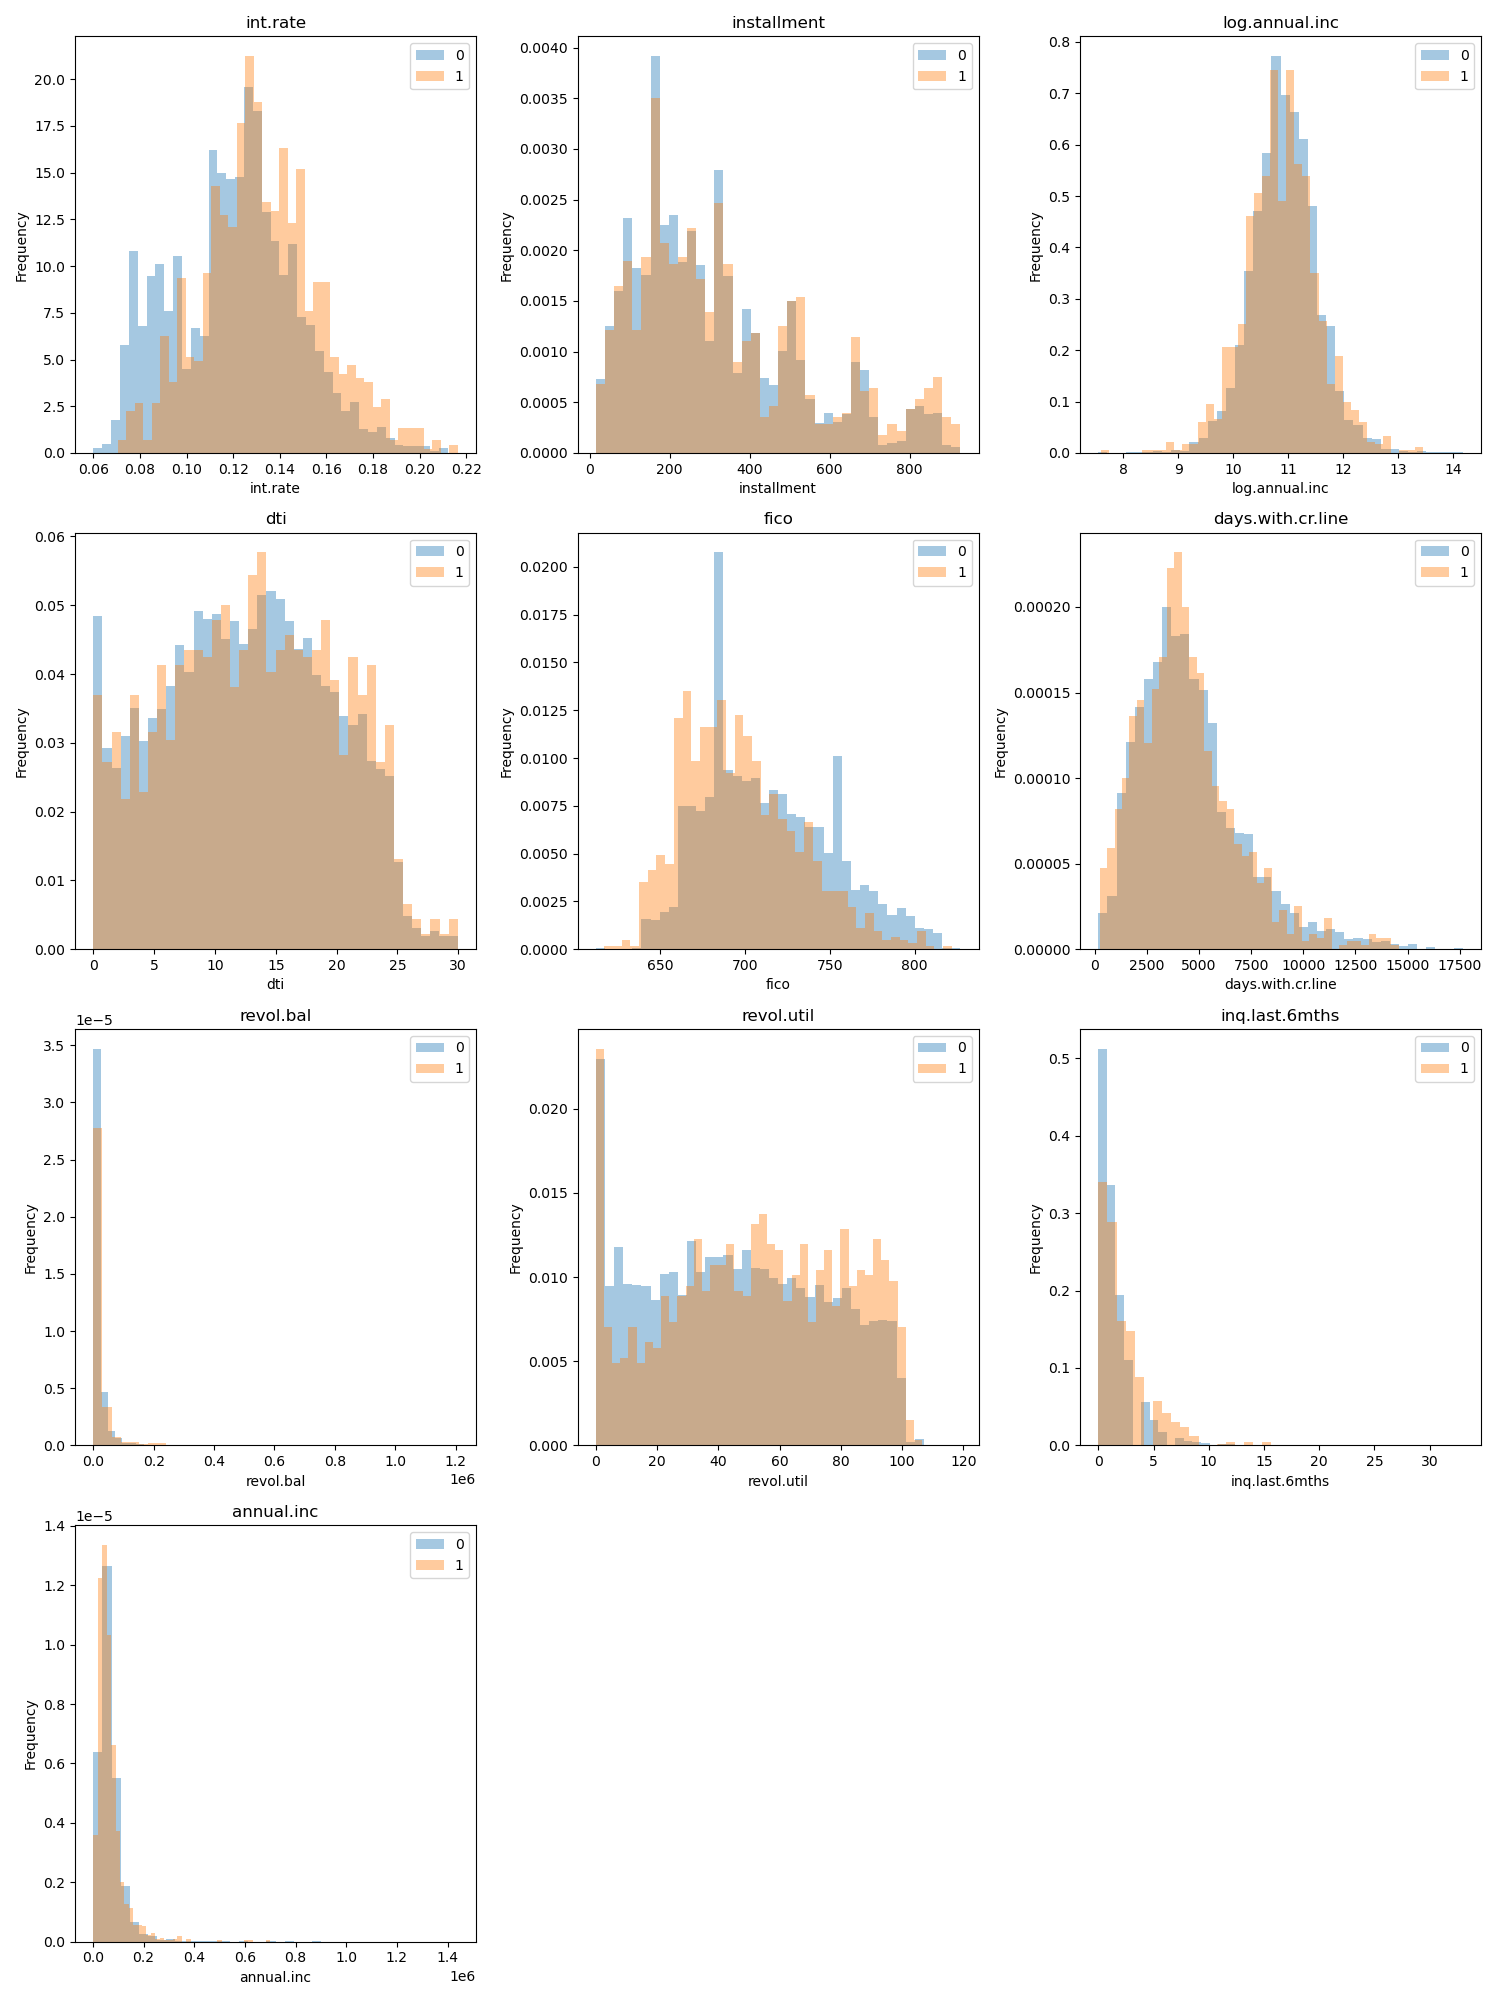
\includegraphics[width=1.2\textwidth,height=\textheight]{../results/figures/histograms_grid.png}

}

\caption{\label{fig-feature_dist}Empirical distributions of numerical
features between class \texttt{Defaulted(1)} and
\texttt{Fully\ Paid(0)}}

\end{figure}%

Here are some key metrics and considerations:

\begin{itemize}
\item
  Debt-to-Income Ratio
\item
  Credit Utilization Ratio( revol.util): how much of their revolving
  credit borrowers are using relative to their limit with higher values
  indicating possible financial strain.
\item
  Loan Duration vs.~Risk: If longer-term loans are associated with
  higher default rate (days.with.cr.line).
\end{itemize}

\subsubsection{4.1.1 Loan categories}\label{loan-categories}

Below, to help us create the loan categories, we are using the FICO risk
profile categories (Consumer Financial Protection Bureau 2024) See also
(myFICO 2024) and (Equifax 2024) for details on different ranges of
credit.

\begin{itemize}
\item
  Deep subprime (credit scores below 580)
\item
  Subprime (credit scores of 580-619)
\item
  Near-prime (credit scores of 620-659)
\item
  Prime (credit scores of 660-719)
\item
  Super-prime (credit scores of 720 or above)
\end{itemize}

Categorical features like purpose also provided significant insights
(Figure~\ref{fig-purpose_risk}): loans categorized under ``small
business'' and ``credit card'' showed higher default rates compared to
others, such as ``home improvement.''

\begin{figure}

\centering{

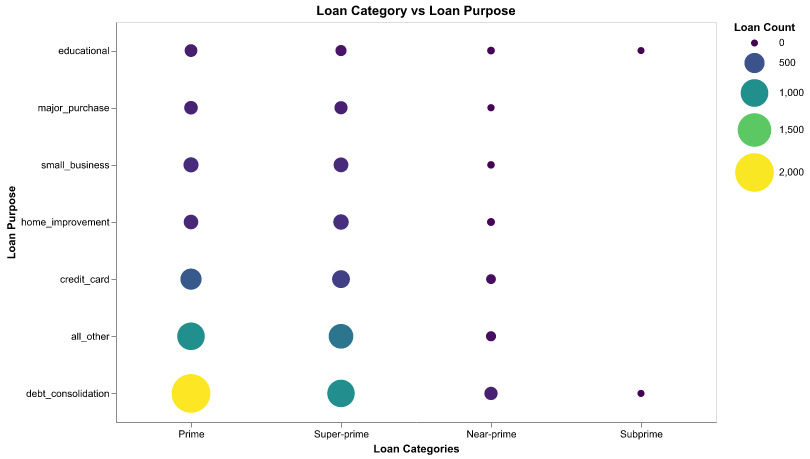
\includegraphics[width=1\textwidth,height=\textheight]{../results/figures/loan_category_vs_purpose.png}

}

\caption{\label{fig-purpose_risk}Distribution of borrower's loan purpose
by their risk profile category}

\end{figure}%

\subsubsection{4.1.2 Risk categories}\label{risk-categories}

Let us explore the data further with specific borrower risk profile
categories. Based on the above five loan categories, we framed three
main risk categories as high, medium and low-risk profiles with:

\begin{itemize}
\item
  Low Risk: credit score of at least 720
\item
  Medium Risk: credit score between 650 and 720
\item
  High Risk: credit score of 650.
\end{itemize}

\begin{figure}

\centering{

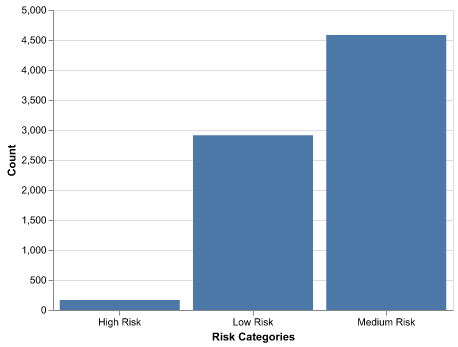
\includegraphics[width=0.6\textwidth,height=\textheight]{../results/figures/risk_categories_distribution.png}

}

\caption{\label{fig-risk_dist}Bar Chart showing the distribution of
borrower's risk level}

\end{figure}%

From Figure~\ref{fig-risk_dist}, we observed a high concentration of
loans in the medium-risk category and a significant number of low-risk
borrowers compared to the high-risk borrowers.

\newpage

\subsubsection{4.1.3 Descriptive Analysis}\label{descriptive-analysis}

~

\begin{figure}

\centering{

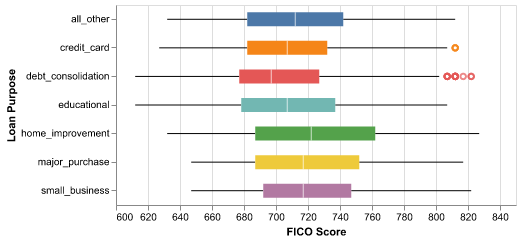
\includegraphics[width=0.8\textwidth,height=\textheight]{../results/figures/boxplot_purpose.png}

}

\caption{\label{fig-fico_purpose}Boxplot comparing borrower's credit
score by their loan purpose}

\end{figure}%

From Figure~\ref{fig-fico_purpose}, we see that the low-risk borrowers
have a lower average debt-to-income ratio as compared to the borrowers
with medium and high-risk profiles, based on their fico score. Note also
the outliers in FICO scores for the loan purpose of debt consolidation
type.

\begin{figure}

\centering{

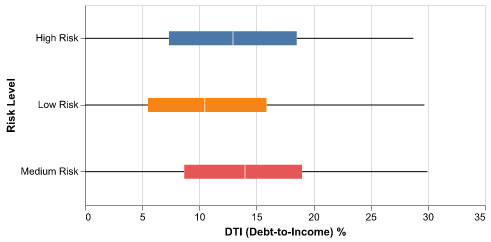
\includegraphics[width=0.7\textwidth,height=\textheight]{../results/figures/boxplot_risk.png}

}

\caption{\label{fig-dti_risk}Boxplot comparing borrower's debt-to-income
ratio by their risk level}

\end{figure}%

From Figure~\ref{fig-dti_risk}, we see that the low risk borrowers have
lower average debt-to-income-ratio as compared to the borrowers with
medium and high risk profile, based on their fico score. Note also the
outliers in FICO scores for the loan purpose of debt consolidation type.

\newpage

\subsubsection{4.1.4 Correlation Analysis}\label{correlation-analysis}

The EDA for most of the numerical columns produces no strong general
trends. We see a higher correlation level between fico and revo.util,
and that of fico and interest rate. (Figure~\ref{fig-corr_map})

\begin{figure}

\centering{

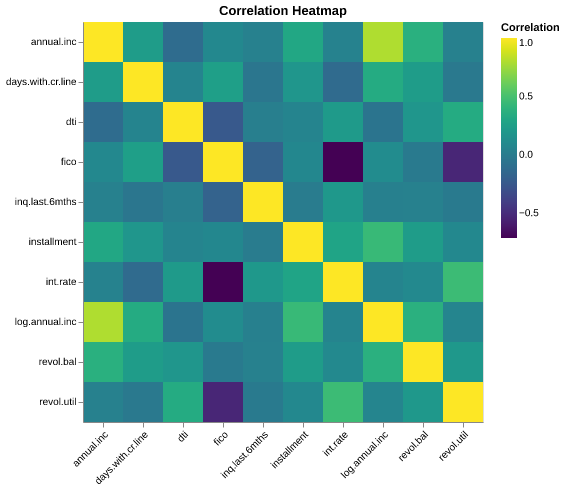
\includegraphics[width=1\textwidth,height=\textheight]{../results/figures/correlation_heatmap.png}

}

\caption{\label{fig-corr_map}Heatmap showing correlation between
features for the lending club data}

\end{figure}%

\subsection{\texorpdfstring{4.2 Model Building
}{4.2 Model Building  }}\label{model-building}

\subsubsection{4.2.1 Data Splitting}\label{data-splitting}

The dataset was split into training (80\%) and test (20\%) sets,
resulting in 1916 observations in the test set. All numeric features
were standardized using standardscaler, while categorical features were
preprocessed using one-hot encoding before model fitting. Any missing
values were imputed using the median for numeric features or the most
frequent value for categorical features.

\subsubsection{4.2.2 Classification
Metrics}\label{classification-metrics}

We decided to use the accuracy score as the classification metric. In
financial decision-making, while false negatives impose greater
financial risk to the platform, false positives can impose great
financial strain on the borrower. Therefore, it is essential to identify
both defaulted and fully paid loans correctly.

\subsubsection{4.2.3 Model Selection}\label{model-selection}

To decide on the most suitable classification model to build on, we have
conducted a 10-fold cross-validation on four different classification
models: DecisionTree, kNN-neighbours, SVC, and Logistic Regression.

\begin{longtable}[]{@{}
  >{\raggedright\arraybackslash}p{(\columnwidth - 6\tabcolsep) * \real{0.2500}}
  >{\raggedright\arraybackslash}p{(\columnwidth - 6\tabcolsep) * \real{0.2500}}
  >{\raggedright\arraybackslash}p{(\columnwidth - 6\tabcolsep) * \real{0.2500}}
  >{\raggedright\arraybackslash}p{(\columnwidth - 6\tabcolsep) * \real{0.2500}}@{}}

\caption{\label{tbl-cv_results}Cross-validation results of various
classification model.}

\tabularnewline

\toprule\noalign{}
\begin{minipage}[b]{\linewidth}\raggedright
fit\_time
\end{minipage} & \begin{minipage}[b]{\linewidth}\raggedright
score\_time
\end{minipage} & \begin{minipage}[b]{\linewidth}\raggedright
test\_score
\end{minipage} & \begin{minipage}[b]{\linewidth}\raggedright
train\_score
\end{minipage} \\
\midrule\noalign{}
\endhead
\bottomrule\noalign{}
\endlastfoot
0.069(+/-0.006) & 0.002(+/-0.001) & 0.737(+/-0.016) & 1.000(+/-0.000) \\
0.011(+/-0.001) & 0.019(+/-0.029) & 0.823(+/-0.008) & 0.855(+/-0.001) \\
1.009(+/-0.018) & 0.091(+/-0.008) & 0.841(+/-0.002) & 0.845(+/-0.000) \\
0.020(+/-0.009) & 0.003(+/-0.001) & 0.839(+/-0.003) & 0.840(+/-0.000) \\

\end{longtable}

Table~\ref{tbl-cv_results} shows the mean validation score and training
score for each model. We can see that the decision tree model has a much
smaller cross-validation score compared to the other three models.

While the SVC model has a slightly larger test score than the logistic
model, it requires a significantly longer computation time. Since the
test score for SVC and Logistic Regression is very similar (both being
\textasciitilde0.84), We have opted for the logistic regression model as
our predictor. The train score of the Logistic Regression is the same as
the validation score, suggesting that the model is likely not overfitted
and will be able to generalize well to unseen data.

The logistic Regression Model was selected as the final model to predict
loan default risk due to its simplicity, slightly higher accuracy, and
interpretability. All variables included in the original data set were
used in model fitting.

~ ~

\subsubsection{4.2.4 Hyperparameter
Optimization}\label{hyperparameter-optimization}

To find the optimal model for prediction, we used GridSearch to conduct
10-fold cross-validation over different values of the hyperparameter C.
The regularization strength C is a hyperparameter that controls the
trade-off between bias and variance. A high value of C corresponds to
weaker regularization (less penalty on large coefficients), which might
lead to overfitting, while a low value of C increases regularization and
might underfit the model. We conduct GridSearch on a logarithmic range
from \(10^{-5}\) to \(10^{5}\). The range spanning a few orders of
magnitude will ensure the model neither overfits nor underfits.

The results from the GridSearch were shown below
(Figure~\ref{fig-C_tuning}), with the optimal C value of 0.000687.

\begin{figure}

\centering{

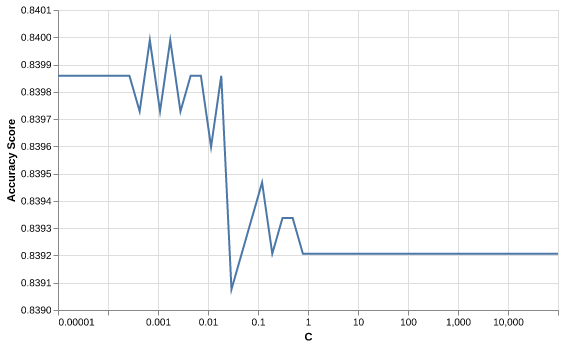
\includegraphics[width=0.7\textwidth,height=\textheight]{../results/figures/param_C_tuning.png}

}

\caption{\label{fig-C_tuning}10-folds cross-validation results for
hyperparameter C tuning. Accuracy score was used as the classification
metric.}

\end{figure}%

\newpage

\section{5. Discussion and
Implications}\label{discussion-and-implications}

\subsection{5.1 Model Evaluation}\label{model-evaluation}

Our model performs well on the test data, achieving a test score of
0.8398.

Here, we identify the top 5 influential features for predicting each
class (Table~\ref{tbl-positive_coef}, Table~\ref{tbl-negative_coef},).
The Logistic Regression's coefficients have provided insights into
feature importance, highlighting predictors such as higher credit score
(\texttt{fico}) and larger income growth(\texttt{log.annual.inc}) to be
associated with lower default risk. Meanwhile, borrowers with higher
loan-to-income ratios, interest rates, and more inquiries in the past 6
months exhibited a greater likelihood of default.

~ ~

\begin{longtable}[]{@{}lr@{}}

\caption{\label{tbl-positive_coef}Top 3 influential feature for
predicting class \texttt{Defaulted(1)}}

\tabularnewline

\toprule\noalign{}
features & positive coefficient \\
\midrule\noalign{}
\endhead
\bottomrule\noalign{}
\endlastfoot
num\_\_fico & -0.1034 \\
num\_\_credit.policy & -0.101 \\
num\_\_log.annual.inc & -0.0533 \\

\end{longtable}

~ ~

\begin{longtable}[]{@{}lr@{}}

\caption{\label{tbl-negative_coef}Top 3 influential feature for
predicting class \texttt{Fully\ Paid(0)}}

\tabularnewline

\toprule\noalign{}
features & negative coefficient \\
\midrule\noalign{}
\endhead
\bottomrule\noalign{}
\endlastfoot
num\_\_int.rate & 0.1193 \\
num\_\_inq.last.6mths & 0.1105 \\
num\_\_installment & 0.0621 \\

\end{longtable}

~ ~

The model correctly predicted 1608 cases out of 1916 on the test set,
with 308 errors as shown in Table~\ref{tbl-confusion_matrix}.

These errors were distributed across false positives and false
negatives. False negatives, representing cases where a defaulted loan
was not flagged, pose a greater financial risk, as these borrowers are
likely to incur losses. False positives, on the other hand, might result
in stricter lending requirements for borrowers who would have
successfully repaid their loans.

~ ~

\begin{longtable}[]{@{}
  >{\raggedright\arraybackslash}p{(\columnwidth - 4\tabcolsep) * \real{0.3011}}
  >{\raggedleft\arraybackslash}p{(\columnwidth - 4\tabcolsep) * \real{0.3441}}
  >{\raggedleft\arraybackslash}p{(\columnwidth - 4\tabcolsep) * \real{0.3548}}@{}}

\caption{\label{tbl-confusion_matrix}Confusion Matrix of Logistic
Regression Model on Test Data}

\tabularnewline

\toprule\noalign{}
\begin{minipage}[b]{\linewidth}\raggedright
\end{minipage} & \begin{minipage}[b]{\linewidth}\raggedleft
Predict Positive (defaulted)
\end{minipage} & \begin{minipage}[b]{\linewidth}\raggedleft
Predict Negative (fully paid)
\end{minipage} \\
\midrule\noalign{}
\endhead
\bottomrule\noalign{}
\endlastfoot
True Positive (defaulted) & 0 & 306 \\
True Negative (fully paid) & 1 & 1609 \\

\end{longtable}

~ ~

Despite the high accuracy score, our model fails to identify any of the
306 actual default loans. This suggests that the accuracy score cannot
fully reflect the model performance. However, our model is a great
predictor in identifying negative loan defaults (over 99\% of the fully
paid cases identified), and the high false negative limits its real-life
application. Further steps are needed to improve the model so that it
can also predict defaulted loans well.

Future work will focus on improving the model's ability to predict
defaults by exploring methods for handling imbalanced datasets. One
approach is to experiment with machine learning models designed to
manage class imbalance better:

\begin{enumerate}
\def\labelenumi{(\arabic{enumi})}
\item
  Data-level Adjustments: Undersampling to Reduce the number of majority
  class instances to balance the dataset; Oversampling: Increasing the
  number of minority class instances to achieve balance; Random
  Oversampling: Duplicating minority class instances at random; SMOTE:
  Generating synthetic examples of the minority class to train the model
  better; and
\item
  Training Procedure Adjustments like Stratified Splits, Class Weight
  Adjustment and Dynamic Resampling.
\end{enumerate}

\subsection{5.2 Limitations}\label{limitations}

\begin{longtable}[]{@{}rr@{}}

\caption{\label{tbl-target_dist}Target distribution showing class
imbalance biased towards class \texttt{Fully\ Paid(0)}}

\tabularnewline

\toprule\noalign{}
not.fully.paid & proportion \\
\midrule\noalign{}
\endhead
\bottomrule\noalign{}
\endlastfoot
0 & 0.839859 \\
1 & 0.160141 \\

\end{longtable}

As we check the distribution of the target, we can see that the
proportion of borrowers who have repaid their loans is significantly
higher than those who defaulted on their loans. The class imbalance of
the target results in the model predicting most cases as ``negative''
(fully paid).

Possible solutions to the high false negtative include adjusting the
\texttt{class\_weight} hyperparameter or adjusting the decision
threshold of the logistic model. Since accuracy might not fully reflect
the model performance in the case of class imbalance, it would be good
to include other evaluation metrics when evaluating model performance. A
good alternative classification metrics would be the F1 score, as it
minimises false positive and false negative while balancing the
precision and recall.

Also, based on the feature importance obtained, additional feature
engineering or feature selection can potentially improve model
performance.

Another alternative is to use a non-linear classification model to
account for possible non-linear decision boundaries. An example is a
decision tree, which can better model complex non-linear decision
boundaries.

\section*{6. Reference}\label{reference}
\addcontentsline{toc}{section}{6. Reference}

\phantomsection\label{refs}
\begin{CSLReferences}{1}{0}
\bibitem[\citeproctext]{ref-cai2016judging}
Cai, Shun, Xi Lin, Di Xu, and Xin Fu. 2016. {``Judging Online
Peer-to-Peer Lending Behavior: A Comparison of First-Time and Repeated
Borrowing Requests.''} \emph{Information \& Management} 53 (7): 857--67.

\bibitem[\citeproctext]{ref-ConsumerBureau}
Consumer Financial Protection Bureau. 2024. \emph{Borrower Risk
Profiles}.
\url{https://www.consumerfinance.gov/data-research/consumer-credit-trends/student-loans/borrower-risk-profiles/}.

\bibitem[\citeproctext]{ref-cocser2019predictive}
Coşer, Alexandru, Monica Mihaela Maer-Matei, and Crişan Albu. 2019.
{``PREDICTIVE MODELS FOR LOAN DEFAULT RISK ASSESSMENT.''} \emph{Economic
Computation \& Economic Cybernetics Studies \& Research} 53 (2).

\bibitem[\citeproctext]{ref-Equifax}
Equifax. 2024. \emph{What Are the Different Ranges of Credit}.
\url{https://www.equifax.com/personal/education/credit/score/articles/-/learn/credit-score-ranges/}.

\bibitem[\citeproctext]{ref-numpy}
Harris, Charles R, K Jarrod Millman, Stéfan J van der Walt, Ralf
Gommers, Pauli Virtanen, David Cournapeau, Eric Wieser, et al. 2020.
{``{Array programming with NumPy}.''} \emph{Nature} 585 (7825): 357--62.
\url{https://doi.org/10.1038/s41586-020-2649-2}.

\bibitem[\citeproctext]{ref-matplotlib}
Hunter, J. D. 2007. {``Matplotlib: A 2D Graphics Environment.''}
\emph{Computing in Science \& Engineering} 9 (3): 90--95.
\url{https://doi.org/10.1109/MCSE.2007.55}.

\bibitem[\citeproctext]{ref-khandani2010consumer}
Khandani, Amir E, Adlar J Kim, and Andrew W Lo. 2010. {``Consumer
Credit-Risk Models via Machine-Learning Algorithms.''} \emph{Journal of
Banking \& Finance} 34 (11): 2767--87.

\bibitem[\citeproctext]{ref-lenz2016peer}
Lenz, Rainer. 2016. {``Peer-to-Peer Lending: Opportunities and Risks.''}
\emph{European Journal of Risk Regulation} 7 (4): 688--700.

\bibitem[\citeproctext]{ref-lendingclub}
matmcreative. 2024. \emph{Lending-Club-Loan-Analysis}.
\url{https://github.com/matmcreative/Lending-Club-Loan-Analysis}.

\bibitem[\citeproctext]{ref-myFICO}
myFICO. 2024. \emph{What's in My FICO® Scores?}
\url{https://www.myfico.com/credit-education/whats-in-your-credit-score\#:~:text=FICO\%20Scores\%20are\%20calculated\%20using,and\%20credit\%20mix\%20(10\%25}.

\bibitem[\citeproctext]{ref-sklearn}
Pedregosa, F., G. Varoquaux, A. Gramfort, V. Michel, B. Thirion, O.
Grisel, M. Blondel, et al. 2011. {``{Scikit-learn: Machine Learning in
Python}.''} \emph{Journal of Machine Learning Research} 12: 2825--30.

\bibitem[\citeproctext]{ref-sutherland2018sharing}
Sutherland, Will, and Mohammad Hossein Jarrahi. 2018. {``The Sharing
Economy and Digital Platforms: A Review and Research Agenda.''}
\emph{International Journal of Information Management} 43: 328--41.

\bibitem[\citeproctext]{ref-pandas}
team, The pandas development. 2020. {``Pandas-Dev/Pandas: Pandas.''}
Zenodo. \url{https://doi.org/10.5281/zenodo.3509134}.

\bibitem[\citeproctext]{ref-Python}
Van Rossum, Guido, and Fred L. Drake. 2009. \emph{Python 3 Reference
Manual}. Scotts Valley, CA: CreateSpace.

\bibitem[\citeproctext]{ref-altair}
VanderPlas, Jake. 2018. {``Altair: Interactive Statistical
Visualizations for Python.''} \emph{Journal of Open Source Software} 3
(7825, 32): 1057. \url{https://doi.org/10.21105/joss.01057}.

\end{CSLReferences}




\end{document}
